\documentclass[12pt,a4paper]{article}

\usepackage[margin=1in]{geometry}
\usepackage{times}
\usepackage[T1]{fontenc}
\usepackage{amsmath,amssymb}
\usepackage{graphicx}
\usepackage{booktabs}
\usepackage{longtable}
\usepackage{array}
\usepackage{multirow}
\usepackage{enumitem}
\usepackage{listings}
\usepackage{xcolor}
\usepackage{float}
\usepackage{caption}
\usepackage{subcaption}
\usepackage{setspace}
\usepackage{titlesec}
\usepackage{pgfplots}
\pgfplotsset{compat=1.18}
\usepackage[hidelinks]{hyperref}

% Center the major section headings (college template convention);
% subsections stay left-aligned.
\titleformat{\section}{\raggedright\Large\bfseries}{\thesection}{1em}{}
\titleformat{\subsection}{\raggedright\large\bfseries}{\thesubsection}{1em}{}
\titleformat{\subsubsection}{\raggedright\normalsize\bfseries}{\thesubsubsection}{1em}{}

\setstretch{1.15}
\sloppy   % tolerate long \texttt identifiers without overflowing the margin
\raggedbottom % let pages end early instead of stretching voids above the footer
\setlength{\intextsep}{8pt plus 2pt minus 2pt} % snugger gap around [H] figures
\setlength{\parindent}{0pt}
\setlength{\parskip}{6pt}

% ---------- Figure helper: uses the image if present, otherwise a placeholder box ----------
\newcommand{\figplaceholder}[3]{% {file}{width}{placeholder text}
  \IfFileExists{#1}{\includegraphics[width=#2]{#1}}{%
    \fbox{\parbox[c][5cm][c]{#2}{\centering\textit{#3}\\[2pt]\small(place \texttt{\detokenize{#1}} here)}}}%
}

% ---------- Code listing style ----------
\lstdefinestyle{py}{
  language=Python,
  basicstyle=\ttfamily\footnotesize,
  keywordstyle=\color{blue!60!black}\bfseries,
  commentstyle=\color{green!40!black}\itshape,
  stringstyle=\color{red!50!black},
  showstringspaces=false,
  breaklines=true,
  frame=single,
  numbers=left,
  numberstyle=\tiny\color{gray},
  xleftmargin=1.5em,
  framexleftmargin=1.5em,
  columns=fullflexible,
  keepspaces=true
}
\lstset{style=py}

\begin{document}

%====================================================================
% TITLE PAGE
%====================================================================
\begin{titlepage}
\centering
{\large\bfseries Department of Computer Engineering\\
St. Francis Institute of Technology\\
University of Mumbai\\
2025--2026\par}

\vspace{1.2cm}
\figplaceholder{logo.png}{4cm}{College logo}
\vspace{1.2cm}

{\large An Elective Mini Project Report on\par}
{\large\bfseries ``SentryMesh --- Detecting IoT Attacks Using an Ensemble Machine Learning Model''\par}

\vspace{1cm}
{\large\bfseries Subject: Machine Learning [CSC701]\par}

\vspace{1cm}
{\large Under the guidance of\par}
{\large\bfseries Prof.\ \textless Guide Name\textgreater\par}

\vspace{1cm}
{\large By\par}
\vspace{0.4cm}

\begin{tabular}{lcc}
\textbf{Name} & \textbf{Roll No} & \textbf{PID}\\[4pt]
Arshvir Singh Kalsi & 65 & 2321\\
Viraj Prabhu & 55 & 232134\\
Ghrani Poojari & 54 & 232134\\
\end{tabular}
\end{titlepage}

%====================================================================
% TABLE OF CONTENTS
%====================================================================
\begin{center}
    \textbf{\Large Table of Contents}
\end{center}

\vspace{0.5cm}

\begin{center}
\renewcommand{\arraystretch}{1.6}

\noindent
\begin{tabular}{|c|p{10.1cm}|c|}
\hline
\textbf{Sr.No} & \multicolumn{1}{c|}{\textbf{Title}} & \textbf{Page No.} \\
\hline
i & Abstract & 3 \\
\hline
ii & List of Figures & 4 \\
\hline
iii & List of Tables & 4 \\
\hline
1 & Introduction & 5 \\
\hline
2 & Literature Review/Related Work & 7 \\
\hline
3 & Proposed Work/ Methodology & 10 \\
\hline
4 & System Architecture & 15 \\
\hline
5 & Implementation Steps/Procedure & 17 \\
\hline
6 & Experimental Setup & 18 \\
\hline
7 & Evaluation and Result/ Result Discussion & 22 \\
\hline
8 & Graphical User Interface & 27 \\
\hline
9 & Code & 32 \\
\hline
10 & Conclusion & 34 \\
\hline
11 & References & 35 \\
\hline
\end{tabular}
\end{center}

\clearpage

%====================================================================
% ABSTRACT
%====================================================================
\begin{center}
    \textbf{\Large ABSTRACT}
\end{center}

IoT devices such as cameras, smart plugs and sensors are now everywhere, but they are
cheap, always online and rarely well protected. This makes them attractive targets for
attackers, and attacks like Denial of Service (DoS) floods, port scanning
(reconnaissance) and password guessing (credential attacks) need to be caught quickly.
These small devices cannot run heavy detection models themselves, so the natural
question is: where should the ``intelligence'' live? The source paper for this project
(Tomer and Sharma, 2022) answers with ``search in the cloud, serve at the fog'': use a
powerful cloud tier to find the best model, and run only that small model on a
lightweight fog gateway close to the devices. This project, SentryMesh, builds a
complete working system around that idea.

The entire system is developed within the Python programming ecosystem, leveraging
libraries such as Scikit-learn, XGBoost, Pandas, NumPy, Joblib, Psutil and Flask. The
cloud tier trains and compares six different classifiers on labeled network traffic:
Logistic Regression, Decision Tree, Random Forest, XGBoost, SVM and a soft-voting
ensemble, using stratified 5-fold cross-validation. Every candidate is measured the
same way: accuracy, macro-F1, Cohen's kappa, MCC, ROC-AUC, model size and prediction
latency. Instead of blindly picking the most accurate model, the system uses a simple,
explainable rule: any model whose macro-F1 is within 2 percentage points of the best
qualifies, and the fastest of those is deployed to the fog tier. PCA is also tested to
see whether shrinking the features is worth it, and the answer is measured rather than
assumed.

The fog tier loads only the small exported model file and classifies simulated gateway
traffic record by record into Benign, DoS, Probing and Authentication classes. An
unsupervised DBSCAN safety net runs alongside it to flag strange, never-seen-before
traffic as ANOMALOUS. The live stream uses a deliberately different data distribution
from training, so the reported live accuracy is a true generalization test.

On a 45,000-flow dataset, XGBoost won deployment with 99.21\% accuracy, macro-F1 of
0.9706, ROC-AUC of 0.9991, a 424\,KB model file and about 0.01\,ms prediction time per
record. It sustained 99.3\% accuracy on the unseen drifted stream, and a dashboard
shows the whole loop --- training, selection, deployment and live detection --- working
end to end. Because these headline numbers come from a synthetic generator, the entire
pipeline was re-validated on the public CIC-IDS-2017 benchmark (2.51 million flows
after deduplication, leakage-safe port-grouped holdout): XGBoost again won the
selection rule with 99.90\% accuracy and macro-F1 0.9967 at 0.005\,ms per record,
while the source paper's KNN+NB+DT ensemble finished last among the ensembles with a
34.6\,MB memory footprint, and a stronger stacked ensemble (XGBoost + Random Forest
blended by a meta-learner) confirmed that learned blending beats vote-averaging but
loses on deployment cost.

\vspace{0.5cm}
\noindent\textbf{Keywords:} IoT security, intrusion detection, ensemble learning,
XGBoost, cloud--fog offloading, DBSCAN, PCA, model selection.

\clearpage

% -------------------------------------------------------------
% LIST OF FIGURES + LIST OF TABLES
% -------------------------------------------------------------
\begin{center}
    \textbf{\Large List of Figures}
\end{center}

\vspace{0.4cm}

\begin{center}
\renewcommand{\arraystretch}{1.15}
\noindent
\begin{tabular}{|c|p{10.1cm}|c|}
\hline
\textbf{Figure No.} & \multicolumn{1}{c|}{\textbf{Title}} & \textbf{Page No.} \\
\hline
1 & Three-tier cloud--fog--thing architecture & 15 \\
\hline
2 & Cloud-to-fog workflow (train $\rightarrow$ select $\rightarrow$ export $\rightarrow$ infer) & 16 \\
\hline
3 & Overview page: counters, deployed model card, live accuracy, fog resources & 28 \\
\hline
4 & Attack-type distribution and traffic-over-time charts & 28 \\
\hline
5 & Traffic over time by class (line styles per class) & 28 \\
\hline
6 & Candidate comparison table with IN BAND outlines and RULE PICK & 29 \\
\hline
7 & Latency vs macro-F1 scatter with shaded tolerance band & 29 \\
\hline
8 & PCA cumulative-variance chart with 95\% target line & 29 \\
\hline
9 & Confusion-matrix heatmap of the deployed model & 30 \\
\hline
10 & DBSCAN window scatter (2D projection, anomalies in red) & 30 \\
\hline
11 & Live feed with predicted class, confidence and latency & 30 \\
\hline
12 & Device classification timeline & 31 \\
\hline
13 & Light and dark theme comparison & 31 \\
\hline
14 & Accuracy comparison of all six candidates & 26 \\
\hline
15 & Macro-F1 score comparison with tolerance band & 26 \\
\hline
16 & Macro precision vs.\ macro recall & 27 \\
\hline
17 & ROC-AUC comparison & 27 \\
\hline
18 & Inference latency comparison (log scale) & 28 \\
\hline
19 & Serialized model size comparison (log scale) & 28 \\
\hline
\end{tabular}
\end{center}

\vspace{0.8cm}

\begin{center}
    \textbf{\Large List of Tables}
\end{center}

\vspace{0.3cm}

\begin{center}
\renewcommand{\arraystretch}{1.15}
\noindent
\begin{tabular}{|c|p{10.1cm}|c|}
\hline
\textbf{Table No.} & \multicolumn{1}{c|}{\textbf{Title}} & \textbf{Page No.} \\
\hline
1 & Literature review summary & 7 \\
\hline
2 & The six candidates, mapped to syllabus modules & 13 \\
\hline
3 & Dataset summary & 19 \\
\hline
4 & Dataset class distribution & 19 \\
\hline
5 & Requirements from the PRD & 21 \\
\hline
6 & Uniform comparison of all candidates (winner in bold) & 22 \\
\hline
7 & PCA full vs reduced comparison & 24 \\
\hline
8 & Requirements versus measured results & 25 \\
\hline
9 & GUI pages and their purpose & 25 \\
\hline
10 & Real-data candidate comparison (CIC-IDS-2017) & 27 \\
\hline
\end{tabular}
\end{center}

\clearpage

%====================================================================
% 1. INTRODUCTION
%====================================================================
\section{Introduction}

\subsection{Introduction}
IoT devices such as home cameras, smart plugs, routers and industrial sensors are now
part of daily life. They are inexpensive, always connected and, unfortunately, often
insecure --- weak default passwords, unpatched firmware and little built-in defense.
Because they are so numerous, they make attractive targets: a successful attack can
recruit thousands of devices into botnets, knock services offline with DoS floods,
quietly scan networks for weaknesses (probing), or steal credentials. Studies of real
IoT deployments regularly find devices attacked within minutes of going online.

A big constraint is that these devices themselves are tiny computers. They cannot host
deep-learning-grade detection pipelines. Sending every packet to the cloud for
analysis adds round-trip latency that defeats real-time detection, while putting heavy
intelligence directly on the gateway is not feasible either. The source paper for this
project, Tomer and Sharma (2022), proposes the ``search in the cloud, serve at the
fog'' split: use the cloud's abundant compute to find the best detection model, then
run only that small model on a fog gateway close to the devices. However, the paper
leaves open questions that a real system must answer: \emph{how} should the best model
be chosen fairly among candidates of very different speed and accuracy, \emph{how}
does the deployed model behave on traffic it has never seen, and \emph{what} catches
attacks that are new?

SentryMesh is our working answer. It is a complete two-tier prototype: a cloud tier
that trains and benchmarks six classifiers under identical conditions and applies an
explicit, explainable selection rule, and a fog tier that loads only the small winning
model and classifies a simulated live traffic stream, with an unsupervised DBSCAN
safety net for never-before-seen attacks and a dashboard that makes the whole loop
visible.

\subsection{Problem Definition}
Deploying intrusion detection for IoT traffic involves a constant trade-off between
accuracy and lightness. Deep or heavy models may catch more attacks, but they are
slower and larger --- unsuitable for a constrained gateway. Light models are fast but
may miss rare attacks, and choosing one of them purely because it is fast can silently
sacrifice detection quality. The difficulty is that ``best'' depends on both
dimensions at once, and a naive pick of either extreme can be wrong.

This project addresses the problem by building a pipeline that trains and benchmarks
several classical ML models in a compute-rich cloud tier, then selects the best
\textbf{accuracy-versus-lightness} trade-off automatically using an explicit rule, and
deploys only that model to a lightweight fog tier that classifies traffic in real
time. Beyond the two-tier split itself, the core research question is: \emph{can a
simple, transparent selection rule --- ``nearly as accurate as the best, but the
fastest of those'' --- replace ad-hoc model choice, and does the model it picks still
generalize to traffic it has never seen?}

\subsection{Prerequisites}
\textbf{Machine Learning Fundamentals}
\begin{itemize}
  \item Understanding of supervised learning for classification: the full workflow
        from data preprocessing and splitting to model training, stratified k-fold
        cross-validation, and evaluation with metrics such as accuracy, precision,
        recall, F1-score, Cohen's kappa and MCC.
\end{itemize}
\textbf{Core Algorithms and Techniques}
\begin{itemize}
  \item Working knowledge of Logistic Regression, Decision Trees, Random Forest,
        gradient boosting (XGBoost), SVM, soft-voting ensembles, PCA for
        dimensionality reduction and DBSCAN clustering.
\end{itemize}
\textbf{Python Programming and Libraries}
\begin{itemize}
  \item Proficient Python programming, with hands-on experience using Scikit-learn,
        XGBoost, Pandas, NumPy, Joblib, Psutil and Flask --- the libraries this
        project is built on.
\end{itemize}
\textbf{Networking Basics}
\begin{itemize}
  \item Familiarity with flow-level traffic features (bytes, packets, durations,
        protocols) and common IoT attack types (DoS, probing, credential attacks).
\end{itemize}

%====================================================================
% 2. LITERATURE REVIEW
%====================================================================
\clearpage
\section{Literature Review/Related Work}

The table below reviews the source paper this project builds on, together with
related published studies and datasets used in this project, all on
machine-learning-based network intrusion detection. For each work we summarize the
system and its findings, and the gap (paucity) that remains.

\begingroup
\footnotesize
\renewcommand{\arraystretch}{1.3}
\begin{longtable}{|c|p{2.3cm}|p{5.8cm}|p{5.0cm}|}
\caption{Literature review summary}\label{tab:lit}\\
\hline
\textbf{Sr. No} & \textbf{Title of the Paper} & \textbf{Description of the System [Findings]} & \textbf{Gaps [Paucity]}\\
\hline
\endfirsthead
\hline
\textbf{Sr. No} & \textbf{Title of the Paper} & \textbf{Description of the System [Findings]} & \textbf{Gaps [Paucity]}\\
\hline
\endhead
\hline
\endfoot
\hline
\endlastfoot
1 & Detecting IoT Attacks Using an Ensemble ML Model (Tomer \& Sharma, 2022) & Three-tier cloud--fog--thing design. The cloud trains every combination of 5 base classifiers (DT, RF, KNN, LR, NB) under voting and stacking (20 runs) on NSL-KDD. Model 8 (KNN+NB+DT voting) won with 1.15\,s execution time and near-ceiling metrics; ``$<$10\% CPU'' for the fog layer on a 3\,GB RAM machine. & Model selection is implicit, not user-adjustable; no live CPU/memory instrumentation; no drift signal; no zero-day (unseen attack) handling; NSL-KDD reflects dated traffic.\\
\hline
2 & XGBoost: A Scalable Tree Boosting System (Chen \& Guestrin, 2016) & Introduced a regularized gradient-boosted tree system with sparsity-aware split finding and cache-aware learning, with state-of-the-art results on large-scale tabular datasets. & Designed for raw accuracy and throughput; gives no guidance on choosing between a fast approximate model and a slower exact one for a constrained deployment target.\\
\hline
3 & Scikit-learn: Machine Learning in Python (Pedregosa et al., 2011) & Unified API for classical ML: classifiers, ensembles, SVM, PCA, DBSCAN, stratified k-fold and all metrics used in this project. Our uniform six-candidate harness is built directly on it. & A library, not a deployment methodology: it provides no automatic rule for choosing which trained model should actually serve live traffic under a latency budget.\\
\hline
4 & A Density-Based Algorithm for Discovering Clusters (Ester et al., 1996) & DBSCAN groups points in dense regions and labels the rest as noise --- without needing the number of clusters in advance. This is what makes it suitable for flagging unknown attack traffic. & Original work is generic clustering; it does not address streaming network data, rolling windows, or integration with a supervised classifier.\\
\hline
5 & TON\_IoT Telemetry Dataset: A New Generation Dataset of IoT and IIoT for Data-Driven Intrusion Detection Systems (Alsaedi et al., 2020) & Introduces the TON\_IoT collection: large IoT/IIoT telemetry, OS-log and network-flow datasets with labeled benign and attack traffic, validated for training and evaluating intrusion-detection models. & Real datasets were not reachable at project run time, so the project falls back to a deterministic synthetic generator (loaders accept both TON\_IoT and CICIoT2023 as drop-ins).\\
\hline
6 & CICIoT2023: A Real-Time Dataset and Benchmark for Large-Scale Attacks in IoT Environment (Neto et al., 2023) & A contemporary real-device IoT traffic dataset (105 devices) with benign traffic and 33 attack types, released with ML benchmarks for intrusion detection. & Same runtime constraint as above; the full dataset also requires more compute than this mini project's scope.\\
\end{longtable}
\endgroup

\subsection{Source Paper in Detail}
Tomer and Sharma (\textit{Future Internet}, 2022) propose a three-tier IoT security
design (thing, fog, cloud). The cloud tier trains every combination of base
classifiers (Decision Tree, Random Forest, KNN, Logistic Regression, Na\"ive Bayes)
under \textbf{voting} and \textbf{stacking}, giving 20 runs. Models are compared on
accuracy, precision, recall, F-measure, kappa, ROC, MCC, error metrics (MAE, RMSE,
RAE, RRSE) and execution time. The fog tier then runs the selected model on a
constrained node.

Key findings that SentryMesh builds on:
\begin{itemize}
  \item \textbf{Model 8 (KNN + Na\"ive Bayes + Decision Tree, voting)} was selected
        primarily on execution time (1.15\,s) with near-ceiling quality metrics ---
        the same shape as SentryMesh's tolerance-band rule.
  \item Stacking was always slower than voting.
  \item The paper claims \textbf{under 10\% CPU} for the fog layer on a 3\,GB RAM machine
        (Core 2 Duo E7400, 2.80\,GHz).
  \item Training used the NSL-KDD train segment as cloud data and the separate test
        segment as fog data --- a genuinely unseen distribution.
  \item The paper applies no extra feature extraction and has no unsupervised tier.
  \item It cites XGBoost at roughly 99.6 AUC; SentryMesh's XGBoost candidate reached
        ROC-AUC 0.9991.
\end{itemize}


%====================================================================
% 3. PROPOSED WORK / METHODOLOGY
%====================================================================
\clearpage
\section{Proposed Work/ Methodology}

\subsection{Overall Approach}
\begin{enumerate}
  \item \textbf{Cloud role (run once or on demand):} ingest data, preprocess, train
        six candidates with stratified 5-fold CV, evaluate every candidate
        identically, apply the selection rule, evaluate PCA, and export the winner.
  \item \textbf{Fog role (run continuously):} load only the exported artifact,
        classify a live stream record by record, and run an unsupervised DBSCAN
        backstop for novel traffic.
\end{enumerate}

\subsection{Datasets}
\textbf{Description:} labeled IoT network flows with 12 features (byte and packet
counts, sizes, timing and protocol) and 4 classes: Benign, DoS, Probing and
Authentication.

\textbf{Source:} loaders prefer TON\_IoT (\texttt{train\_test\_network.csv}), then any
CICIoT2023 partition CSV placed in \texttt{data/}; when neither is available a
deterministic synthetic generator (fixed seed 42) produces realistic flows with a
natural 72/16/8/4\% class imbalance, so the whole system still runs offline.

\textbf{Exploration and loading:} \texttt{sentrymesh/datasets.py} handles loading and
subsampling; the cloud tier trains on a baseline regime while the fog simulator
replays a deliberately drifted regime, mirroring the source paper's
train-file/test-file design.

\subsection{Algorithms}

\subsubsection*{1. Logistic Regression (LR)}
\textbf{Theory}\\
Logistic Regression is a supervised classification algorithm that models the
probability of each class as a logistic function of a linear combination of the input
features. It is fast, interpretable, and a common baseline for tabular
classification. For multiple classes it is used in the multinomial (softmax) form.
\textbf{Formula}\\
For input features $x$, the model computes class probabilities
\begin{equation}
  P(y = k \mid x) = \frac{\exp(w_k^\top x + b_k)}{\sum_{j} \exp(w_j^\top x + b_j)}
\end{equation}
where $w_k$ and $b_k$ are the learned weight vector and bias for class $k$.

\subsubsection*{2. Decision Tree (CART)}
\textbf{Theory}\\
A decision tree classifies a record by asking a sequence of simple yes/no questions
about its features (``is the flow duration below 0.1\,s?''), splitting the data at
each node to reduce impurity. CART trees use the Gini impurity,
$G = 1 - \sum_k p_k^2$, where $p_k$ is the share of class $k$ in a node; the split
chosen at each node is the one that lowers impurity the most. Trees are easy to read
but a single tree overfits, which motivates ensembles.
\textbf{Formula}\\
The Gini impurity of a node $t$:
\begin{equation}
  G(t) = 1 - \sum_{k=1}^{K} p_k^2
\end{equation}
where $K$ is the number of classes and $p_k$ the proportion of class $k$ samples in
node $t$.

\subsubsection*{3. Random Forest}
\textbf{Theory}\\
A Random Forest is a \emph{bagging} ensemble: it trains many decision trees on
bootstrap samples of the data, and each split considers only a random subset of
features. The forest's prediction is the majority vote of its trees. Averaging many
decorrelated trees reduces variance and typically generalizes better than any single
tree.
\textbf{Formula}\\
For $T$ trees, the predicted class is
\begin{equation}
  \hat{y} = \operatorname{mode}\{\, h_1(x), h_2(x), \ldots, h_T(x) \,\}
\end{equation}
where $h_t(x)$ is the prediction of the $t$-th tree.

\subsubsection*{4. Gradient Boosting (XGBoost)}
\textbf{Theory}\\
Boosting builds an ensemble \emph{sequentially}: each new tree is trained to correct
the residual errors of the current ensemble, and the final prediction is a weighted
sum of all trees. XGBoost adds regularization to the objective, making it both
accurate and efficient --- it is the modern workhorse for tabular data.
\textbf{Formula}\\
The ensemble prediction after $M$ rounds is additive:
\begin{equation}
  \hat{y}_i = \sum_{m=1}^{M} f_m(x_i), \qquad
  \mathcal{L} = \sum_i l(y_i, \hat{y}_i) + \sum_m \Omega(f_m)
\end{equation}
where $l$ is the loss and $\Omega(f)$ a penalty on tree complexity that discourages
overfitting.

\subsubsection*{5. Support Vector Machine (SVM)}
\textbf{Theory}\\
SVM is a supervised learning algorithm used for classification. Its objective is to
find the optimal hyperplane that best separates data points of different classes in a
high-dimensional space. The ``optimal'' hyperplane is the one with the maximum margin
--- the largest distance between the hyperplane and the nearest data points from any
class. These nearest points are called ``support vectors'' because they support or
define the position of the hyperplane. For data that is not linearly separable, SVM
uses the ``kernel trick'' to project the data into a higher dimension where a
separating hyperplane can be found.
\textbf{Formula}\\
For a linearly separable dataset, SVM solves the following optimization problem:
\begin{equation}
  \min_{w,b} \; \frac{1}{2}\lVert w \rVert^2
  \quad\text{subject to}\quad
  y_i(w^\top x_i + b) \ge 1 \;\; \forall i
\end{equation}
where $x_i$ is the feature vector of the $i$-th record, $y_i$ its class label, $w$
the normal vector to the hyperplane and $b$ a bias term. The term $\lVert w\rVert^2$
is what is minimized to maximize the margin.

\subsubsection*{6. Voting Ensemble (Soft Voting)}
\textbf{Theory}\\
Ensemble learning is a technique where multiple models (often called ``base
learners'') are trained to solve the same problem and their predictions are combined
to get a better overall prediction. The idea is that different models may capture
different aspects of the data, and by combining them, their strengths are amplified
while their weaknesses are averaged out. Soft voting specifically combines models by
averaging the prediction probabilities from each model, which respects each model's
confidence rather than treating every vote equally.
\textbf{Formula}\\
The predicted class label $\hat{y}$ is chosen by finding the class with the maximum
averaged probability across all models:
\begin{equation}
  \hat{y} = \arg\max_{j} \; \frac{1}{M} \sum_{i=1}^{M} p_{ij}
\end{equation}
where $M$ is the number of models in the ensemble and $p_{ij}$ is the probability
predicted by the $i$-th model for the $j$-th class. Our ensemble soft-votes Logistic
Regression, Decision Tree and XGBoost.

\subsubsection*{7. Principal Component Analysis (PCA)}
\textbf{Theory}\\
PCA is an unsupervised dimensionality-reduction technique. Its main goal is to
transform a large set of variables (here, the 12 flow features) into a smaller set of
new variables called ``principal components'' while preserving the maximum possible
information (variance) from the original data. It finds the directions in the data
that have the highest variance. The first principal component (PC1) is the direction
that captures the most variance, the second (PC2) the next most, and so on.
\textbf{Formula}\\
The process starts by computing the covariance matrix $S$ of the data. The core of
PCA is then to solve the eigenvalue/eigenvector problem for this matrix:
\begin{equation}
  S v = \lambda v
\end{equation}
where $S$ is the covariance matrix of the input data, $v$ is an eigenvector of the
covariance matrix (each eigenvector is a principal-component direction) and $\lambda$
is the corresponding eigenvalue (the amount of variance captured by that direction).
The eigenvectors are sorted by eigenvalue in descending order, and the top $k$ are
chosen to form the reduced feature space.

\subsubsection*{8. DBSCAN}
\textbf{Theory}\\
DBSCAN (Density-Based Spatial Clustering of Applications with Noise) groups together
points that are closely packed and marks points that lie alone in low-density regions
as noise. Unlike k-means it does not need the number of clusters in advance --- which
is exactly what we want for spotting \emph{unknown} attack shapes: anything that does
not belong to a dense, familiar cluster is flagged as ANOMALOUS. It runs on a rolling
window of 1,500 standardized records ($\varepsilon = 1.8$, min\_samples $= 8$),
re-clustered every 25 records.
\textbf{Formula}\\
A point $p$ is a \emph{core point} if at least \texttt{min\_samples} points lie
within distance $\varepsilon$ of it:
\begin{equation}
  |N_\varepsilon(p)| = |\{\, q : d(p,q) \le \varepsilon \,\}| \;\ge\; \texttt{min\_samples}
\end{equation}
Points reachable from core points form clusters; the rest are noise (ANOMALOUS).

\subsection{Candidate Classifiers}
Table~\ref{tab:candidates} lists the six candidate classifiers used in the
SentryMesh pipeline, along with their algorithmic family and the corresponding
CSC701 syllabus module.

\begin{table}[H]
\caption{The six candidates, mapped to syllabus modules}
\label{tab:candidates}
\centering
\small
\begin{tabular}{p{3.8cm}p{4.4cm}p{4.4cm}}
\toprule
\textbf{Candidate} & \textbf{Family} & \textbf{Syllabus Module}\\
\midrule
Logistic Regression & Linear model & M2 -- Regression \& Trees\\
Decision Tree (CART/Gini) & Single tree & M2\\
Random Forest & Bagging ensemble & M3 -- Ensemble Learning\\
Gradient Boosting (XGBoost) & Boosting ensemble & M3\\
SVM (RBF kernel) & Kernel method & M4 -- Classification\\
Voting Ensemble (LR+DT+XGB) & Soft vote of three base learners & M3 -- combining classifiers\\
\bottomrule
\end{tabular}
\end{table}

\subsection{Model Selection Rule}
The core argument of the project is the following rule:
\begin{quote}
\itshape Among all candidates whose macro-F1 is within 2 percentage points of the
best, deploy the one with the lowest inference latency.
\end{quote}
\begin{itemize}
  \item The band (0--10 pp, default 2) is adjustable in the UI and recomputes
        instantly with no retraining.
  \item Tiebreakers: lowest inference latency, smallest model size, highest raw
        accuracy, or highest Cohen's kappa.
  \item The reasoning (who qualified, who was excluded and why, which tiebreaker
        decided) is stored in \texttt{artifacts/training\_result.json} and shown in
        sentences on the Model Lab page.
  \item \textbf{Rationale:} the band rewards light models that are \textit{nearly as
        accurate}; it does not crown the cheapest model regardless of accuracy.
\end{itemize}

Formally, with $F_c$ the macro-F1 of candidate $c$, tolerance $\tau$ and tiebreaker
cost $t(c)$:
\begin{equation}
  Q = \{\,c : F_c \ge \max_k F_k - \tau\,\}, \qquad
  c^{*} = \arg\min_{c\in Q}\, t(c)
\end{equation}

\subsection{Uniform Evaluation Harness}
Every candidate receives the identical evaluation: confusion matrix, per-class
precision/recall/F1, macro-F1, Cohen's kappa, MCC, ROC-AUC (one-vs-rest), a
Weka-style error suite (MAE/RMSE/RAE/RRSE), serialized model size and batch-averaged
per-record latency. Training uses stratified 5-fold cross-validation.

%====================================================================
% 4. SYSTEM ARCHITECTURE
%====================================================================
\clearpage
\section{System Architecture}

\subsection{Three Tiers}
\begin{figure}[H]
  \centering
  \figplaceholder{images/fig1_architecture.png}{\textwidth}{Three-tier architecture: Thing / IoT traffic $\rightarrow$ Fog (real-time inference) $\Leftrightarrow$ Cloud (model search and training)}
  \caption{Three-tier cloud--fog--thing architecture}
  \label{fig:arch}
\end{figure}

\begin{itemize}
  \item \textbf{Thing layer:} IoT devices generating traffic; simulated from the
        dataset in this version (live capture is future work).
  \item \textbf{Fog layer:} a lightweight service loading only the exported winner;
        it classifies each record, reports confidence and per-record latency, and
        samples its own CPU/RSS/threads.
  \item \textbf{Cloud layer:} ingests labeled traffic, trains and scores all
        candidates, applies the selection rule and exports a portable artifact.
\end{itemize}

\subsection{Data and Control Flow}
\begin{enumerate}
  \item Dataset loaded (TON\_IoT \texttt{train\_test\_network.csv}, CICIoT2023
        partition, or synthetic fallback).
  \item Cloud sweep: 6 candidates $\times$ 5-fold CV $\rightarrow$ metrics table.
  \item Selection rule and PCA decision $\rightarrow$ winner.
  \item Export to \texttt{artifacts/deployed\_model.joblib} (pipeline, class map,
        trained-on metadata, selection reasoning).
  \item The edge engine loads the artifact; the simulator streams records; the engine
        classifies, tracks live accuracy and runs DBSCAN every 25 records.
  \item A REST API feeds the single-page dashboard.
\end{enumerate}

\begin{figure}[H]
  \centering
  \figplaceholder{images/fig2_workflow.png}{\textwidth}{Cloud-to-fog workflow: train $\rightarrow$ select $\rightarrow$ export $\rightarrow$ infer}
  \caption{Cloud-to-fog workflow}
  \label{fig:workflow}
\end{figure}

\subsection{Deployment Modes}
\begin{itemize}
  \item \textbf{Rule automatic:} the artifact is the rule's pick.
  \item \textbf{Manual override:} any candidate can be deployed from the comparison
        table (refit on the stored split, artifact swapped, banner flips to MANUAL
        OVERRIDE) and reset back with one click.
  \item \textbf{Variant toggle:} \texttt{full\_features} or \texttt{pca\_reduced}.
\end{itemize}

\subsection{Software Components}
The project is organized as follows:
\begin{lstlisting}[language={},numbers=none,basicstyle=\ttfamily\scriptsize]
SentryMesh/
|-- run.py                     # entry point (python run.py)
|-- train.py                   # standalone cloud-role training run
|-- sentrymesh/
|   |-- datasets.py            # TON_IoT / CICIoT2023 / synthetic loaders
|   |-- cloud.py               # training, evaluation, selection, PCA, export
|   |-- edge.py                # deployed-model engine, simulator, DBSCAN
|   `-- app.py                 # Flask REST API + static hosting
|-- static/
|   |-- index.html             # SPA shell
|   |-- app.js                 # five pages, client-rendered
|   `-- style.css              # monochrome design system
|-- artifacts/
|   |-- deployed_model.joblib  # winning pipeline (edge loads only this)
|   `-- training_result.json   # full run record
`-- data/                      # optional real-dataset drop-in
\end{lstlisting}

%====================================================================
% 5. IMPLEMENTATION
%====================================================================
\clearpage
\section{Implementation Steps/Procedure}

\begin{enumerate}
  \item \textbf{Dataset ingestion and preprocessing.} Loaders in \texttt{datasets.py}
        prefer TON\_IoT, then CICIoT2023, otherwise use the deterministic synthetic
        generator (fixed seed 42, realistic 72/16/8/4\% class imbalance). Subsampling
        and a stratified 75/25 train/test split are applied; no oversampling.
  \item \textbf{Feature engineering (synthetic flows, 12 features).} Flow shape
        (byte/packet totals, per-packet bytes, byte and packet ratios, inter-arrival
        time), response-side behaviour, and protocol code (TCP/UDP/ICMP). Attack
        profiles: DoS = floods with near-zero duration; Probing = many tiny
        short-lived connections; Authentication = repeated moderate credential
        exchanges.
  \item \textbf{Cloud sweep.} Train the six candidates with stratified 5-fold CV;
        evaluate each with the uniform harness; measure latency (500-record batch, 5
        repetitions) and size (joblib, compression 3).
  \item \textbf{Selection.} Apply the tolerance-band rule and tiebreaker; record the
        sentence-level reasoning.
  \item \textbf{PCA evaluation.} Fit PCA (at least 95\% variance), re-evaluate the
        winner, apply the adoption rule, and choose the full or reduced variant.
  \item \textbf{Export.} Serialize the winning pipeline plus metadata to
        \texttt{artifacts/deployed\_model.joblib}.
  \item \textbf{Edge engine.} Load the artifact only; classify streamed records;
        measure per-record latency; run DBSCAN every 25 records on the rolling
        window; compute live accuracy from carried true labels; sample CPU/RSS/threads
        every 2\,s using \texttt{psutil}.
  \item \textbf{Traffic simulator.} Replays the drifted stream with 50\,ms pacing;
        speed presets 1x / 5x / 20x correspond to 20 / 100 / 400 records per second.
  \item \textbf{API and dashboard.} Flask REST endpoints plus a static single-page
        app with five pages.
\end{enumerate}

\textbf{How to run}
\begin{lstlisting}[language={},numbers=none]
pip install flask scikit-learn pandas numpy joblib xgboost
python train.py      # optional: standalone cloud role, rewrites artifacts/*
python run.py        # serves the app on http://127.0.0.1:5000
\end{lstlisting}
In the UI: \textbf{Model Lab $\rightarrow$ Train Models} (a few minutes), then
\textbf{Live Detection $\rightarrow$ Start simulator}.

%====================================================================
% 6. EXPERIMENTAL SETUP
%====================================================================
\clearpage
\section{Experimental Setup}

\subsection{Parameters}
\begin{description}[leftmargin=1em,style=nextline]
  \item[n\_rows: 45,000] Total synthetic flows generated. Large enough for stable
        metrics on a 4-class problem, small enough to train all six candidates in a
        few minutes on a laptop.
  \item[test\_split: 0.25] Share of data held out for final testing (11,250 records),
        stratified so class proportions are preserved.
  \item[random\_state: 42] Seed for all random processes --- data generation, splits
        and model initializations --- making every result reproducible.
  \item[cv\_folds: 5] Stratified 5-fold cross-validation, giving a more reliable
        estimate than a single split by averaging over 5 different train/test
        subsets.
  \item[tolerance: 0.02] The selection band: candidates within 2 percentage points
        of the best macro-F1 qualify for deployment.
  \item[latency: 500 rec $\times$ 5 reps] Inference latency is averaged over a
        500-record batch, repeated 5 times.
  \item[pca\_variance\_target: 0.95] PCA must retain at least 95\% of the variance
        to be considered.
  \item[dbscan: eps = 1.8, min\_samples = 8] Applied to a rolling window of 1,500
        standardized records, re-clustered every 25 records.
  \item[simulator\_pacing: 50\,ms] Base replay speed; presets 1x/5x/20x correspond to
        20/100/400 records per second.
\end{description}

\subsection{Dataset}
Table~\ref{tab:dataset} summarizes the dataset used for the primary deployment study,
and Table~\ref{tab:classdist} shows the class distribution.

\begin{table}[H]
\caption{Dataset summary}
\label{tab:dataset}
\centering
\small
\begin{tabular}{p{2.6cm}p{10.4cm}}
\toprule
\textbf{Item} & \textbf{Detail}\\
\midrule
Source & Deterministic synthetic IoT-flow generator (offline fallback)\\
Reason & TON\_IoT and CICIoT2023 were not reachable at run time; loaders accept both as drop-in files and prefer them automatically. The CIC-IDS-2017 benchmark was later obtained locally and powers the real-data validation study of Section~7.4\\
Rows & 45,000 flows, 12 features\\
Split & 75\% train / 25\% stratified test (11,250 held-out records)\\
Seed & 42 (fully reproducible)\\
\bottomrule
\end{tabular}
\end{table}

\begin{table}[H]
\caption{Dataset class distribution (natural imbalance preserved)}
\label{tab:classdist}
\centering
\small
\begin{tabular}{lrr}
\toprule
\textbf{Class} & \textbf{Rows} & \textbf{Share}\\
\midrule
Benign & 32,513 & 72.3\%\\
DoS & 7,092 & 15.8\%\\
Probing & 3,604 & 8.0\%\\
Authentication & 1,791 & 4.0\%\\
\bottomrule
\end{tabular}
\end{table}

\subsection{Evaluation Protocol}
\begin{itemize}
  \item Stratified 5-fold cross-validation (CV macro-F1 $\pm$ standard deviation
        reported).
  \item Latency: mean over a 500-record batch, 5 repetitions.
  \item Size: serialized joblib artifact (compression 3).
  \item Precision/recall are macro-averaged across the four classes; per-class recall
        is used as the sensitivity measure.
  \item The error suite is computed from predicted probabilities.
\end{itemize}

\subsection{Libraries}
\begin{description}[leftmargin=1em,style=nextline]
  \item[Scikit-learn] \textbf{Purpose:} classical ML models, cross-validation and
    evaluation. \textbf{Key components used:} \texttt{LogisticRegression},
    \texttt{DecisionTreeClassifier}, \texttt{RandomForestClassifier}, \texttt{SVC},
    \texttt{VotingClassifier}, \texttt{PCA}, \texttt{DBSCAN},
    \texttt{StratifiedKFold}, \texttt{accuracy\_score},
    \texttt{classification\_report}, \texttt{confusion\_matrix},
    \texttt{cohen\_kappa\_score}, \texttt{matthews\_corrcoef}.
  \item[XGBoost] \textbf{Purpose:} the gradient-boosting candidate (the eventual
    winner). \textbf{Key components used:} \texttt{XGBClassifier} with a fixed seed.
  \item[Pandas \& NumPy] \textbf{Purpose:} data loading, manipulation and numerical
    computation. \textbf{Key components used:} \texttt{pd.read\_csv},
    \texttt{pd.DataFrame}, array operations.
  \item[Joblib] \textbf{Purpose:} model persistence. \textbf{Key components used:}
    \texttt{joblib.dump} (compression 3) to export the deployed pipeline and
    \texttt{joblib.load} at the fog tier.
  \item[Psutil] \textbf{Purpose:} fog-node resource instrumentation. \textbf{Key
    components used:} \texttt{psutil.Process().cpu\_percent()}, RSS memory and
    thread count, sampled every 2\,s.
  \item[Flask] \textbf{Purpose:} REST API and static hosting of the dashboard.
    \textbf{Key components used:} \texttt{Flask}, \texttt{jsonify}, static file
    serving.
\end{description}

\subsection{Languages}
The entire project is implemented in Python --- the industry standard for machine
learning. Python offers a rich ecosystem of open-source ML libraries (all listed
above), clean and readable syntax that speeds up experimentation, and strong
cross-platform portability: the project runs unchanged on Windows, macOS and Linux.

\subsection{Runtime Environment}
A single-machine prototype: the fog process shares the host with the Flask server,
dataset and charts. The paper's constrained-hardware setup (3\,GB RAM, Core 2 Duo
E7400) was not reproduced; a Raspberry Pi-class run is future work.

\subsection{Requirements from the PRD}
Table~\ref{tab:prd} lists the performance and operational requirements derived from
the product requirements document.

\begin{table}[H]
\caption{Requirements from the PRD}
\label{tab:prd}
\centering
\small
\begin{tabular}{p{3.2cm}p{9.5cm}}
\toprule
\textbf{Requirement} & \textbf{Target}\\
\midrule
Held-out accuracy & $\ge$ 99\%\\
ROC-AUC & $\ge$ 0.99\\
Fog inference & $<$ 2\,s per batch ($\le$ 1.5\,s per inference batch as success metric)\\
Fog CPU & $<$ 10\% on a constrained node\\
Reproducibility & Fixed random seed\\
Portability & Artifact loads without the cloud training stack\\
End to end & Cloud$\rightarrow$fog handoff with no manual intervention\\
\bottomrule
\end{tabular}
\end{table}

%====================================================================
% 7. EVALUATION AND RESULTS
%====================================================================
\clearpage
\section{Evaluation and Results}

\subsection{Performance Metrics}
To evaluate the candidates fairly --- especially with imbalanced classes (only 4\%
Authentication traffic) --- we used:
\begin{itemize}
  \item \textbf{Accuracy}: overall share of records classified correctly.
  \item \textbf{Macro-averaged Precision, Recall and F1}: computed per class and
        averaged, so rare classes count as much as frequent ones.
  \item \textbf{Cohen's kappa and MCC}: agreement and correlation measures that
        correct for chance, more honest than raw accuracy under imbalance.
  \item \textbf{ROC-AUC (one-vs-rest)}: ranking quality of predicted probabilities.
  \item \textbf{Model size and inference latency}: the deployment-cost dimensions of
        the selection rule.
\end{itemize}

\subsection{Model Comparison}
All six candidates were evaluated on the same 11,250-record held-out test set. The
results are in Table~\ref{tab:compare}; the deployed model is XGBoost.

\begin{table}[H]
\caption{Uniform comparison of all candidates (winner in bold)}
\label{tab:compare}
\centering
\scriptsize
\setlength{\tabcolsep}{3pt}
\resizebox{\textwidth}{!}{%
\begin{tabular}{llccccccccc}
\toprule
\textbf{Candidate} & \textbf{Mod.} & \textbf{Acc.} & \textbf{macro-F1} & \textbf{Prec.} & \textbf{Recall} & \textbf{Kappa} & \textbf{MCC} & \textbf{ROC-AUC} & \textbf{Size} & \textbf{Lat. (ms/rec)}\\
\midrule
Logistic Regression & M2 & 0.9738 & 0.8917 & 0.9488 & 0.8597 & 0.9394 & 0.9405 & 0.9912 & 1.5\,KB & 0.0031\\
Decision Tree & M2 & 0.9862 & 0.9500 & 0.9621 & 0.9393 & 0.9688 & 0.9689 & 0.9687 & 15.7\,KB & 0.0027\\
Random Forest & M3 & 0.9893 & 0.9600 & 0.9795 & 0.9438 & 0.9758 & 0.9759 & 0.9982 & 2,571\,KB & 0.0913\\
\textbf{XGBoost} & \textbf{M3} & \textbf{0.9921} & \textbf{0.9706} & \textbf{0.9867} & \textbf{0.9566} & \textbf{0.9821} & \textbf{0.9822} & \textbf{0.9991} & \textbf{424\,KB} & \textbf{0.0078}\\
SVM (RBF) & M4 & 0.9746 & 0.9002 & 0.9538 & 0.8671 & 0.9412 & 0.9423 & 0.9806 & 269\,KB & 0.4018\\
Voting (LR+DT+XGB) & M3 & 0.9901 & 0.9629 & 0.9856 & 0.9443 & 0.9776 & 0.9778 & 0.9976 & 441\,KB & 0.0142\\
\bottomrule
\end{tabular}}
\end{table}

\textbf{Precision/recall diagnosis.} XGBoost and the Voting Ensemble keep both
precision and recall above 0.95: they catch attacks and rarely raise false alarms.
Logistic Regression and SVM show the classic imbalance pattern: precision of about
0.95 but recall of only about 0.86, meaning they miss roughly one in seven attack
records, mostly in the rare Authentication class.

\textbf{Error suite (deployed XGBoost, full features):} MAE 0.0048, RMSE 0.0571, RAE
0.0216, RRSE 0.1713. This is an order of magnitude better than the zero-R baseline on
RAE. The SVM's weak probability calibration (MAE 0.1582) explains why
its error cells dominate the suite even where its hard-label metrics look acceptable.

\subsection{Selection Reasoning}
\begin{itemize}
  \item Best macro-F1 is \textbf{0.9706} (XGBoost). The band threshold is $\ge
        0.9506$, so \textbf{3 of 6 candidates qualified}: Random Forest (0.9600),
        XGBoost (0.9706) and the Voting Ensemble (0.9629).
  \item Latency tiebreaker: XGBoost 0.0078\,ms versus Voting 0.0142\,ms versus Random
        Forest 0.0913\,ms, so \textbf{XGBoost wins} (about 2$\times$ cheaper than the
        vote and about 12$\times$ cheaper than the forest).
  \item Excluded: Logistic Regression (0.8917), Decision Tree (0.9500, just 0.0006
        short of the band) and SVM (0.9002).
  \item The run shows both sides of the rule: the Decision Tree was cheapest of all
        (0.0027\,ms) but missed the band, so cheapness alone did not win; Random
        Forest and the Voting Ensemble met the band but lost on latency.
  \item The Voting Ensemble (the paper's core technique) placed 3rd on latency among
        the qualified and 2nd on kappa, supporting the paper's finding that combining
        classifiers buys robustness at extra execution cost.
\end{itemize}

\subsection{Real-Data Validation on CIC-IDS-2017}
Because the headline results above are synthetic, the whole pipeline was re-run on a
public benchmark: CIC-IDS-2017 (Sharafaldin \textit{et al.}~\cite{ref9}), using all
eight working-day files totalling 2{,}830{,}743 flows. Three preprocessing steps were
applied: label mapping to the project taxonomy (BENIGN $\rightarrow$ Benign,
DDoS/DoS $\rightarrow$ DoS, PortScan $\rightarrow$ Probing; 18{,}028 Bot and
Infiltration flows excluded as out-of-taxonomy), exact-duplicate removal (303{,}648
rows, a known accuracy-inflation source in this benchmark), and twelve flow-shape
features matching the synthetic schema. Evaluation used a leakage-safe split: flows
were grouped by destination port (high-volume ports such as 80/443/53 sharded twenty
ways so a campaign cannot sit entirely on one side), the holdout was drawn per class
so every class is guaranteed present on both sides, and training used a stratified
600{,}000-flow subsample. The final split is 600{,}000 train versus 510{,}963 test
flows (Benign 428{,}826, DoS 63{,}907, Probing 18{,}230). The source paper's
KNN+NB+DT ensemble was trained alongside a stronger stacked generalization (XGBoost
+ Random Forest blended by a logistic-regression meta-learner); SVM was dropped as
computationally prohibitive at this scale. Table~\ref{tab:realcompare} reports the
outcome.

\begin{table}[H]
\caption{Real-data candidate comparison on CIC-IDS-2017 (deduplicated, class-stratified port-grouped holdout, $n_{test}=510{,}963$; winner in bold)}
\label{tab:realcompare}
\centering
\scriptsize
\setlength{\tabcolsep}{3pt}
\resizebox{\textwidth}{!}{%
\begin{tabular}{lccccccc}
\toprule
\textbf{Candidate} & \textbf{Acc.} & \textbf{macro-F1} & \textbf{Prec.} & \textbf{Recall} & \textbf{Kappa} & \textbf{Size} & \textbf{Lat. (ms/rec)}\\
\midrule
Logistic Regression & 0.9343 & 0.7337 & 0.8283 & 0.6778 & 0.7303 & 1.6\,KB & 0.003\\
Decision Tree (CART/Gini) & 0.9968 & 0.9903 & 0.9911 & 0.9895 & 0.9884 & 52\,KB & 0.003\\
Random Forest (bagging) & 0.9974 & 0.9937 & 0.9924 & 0.9949 & 0.9908 & 6{,}194\,KB & 0.049\\
\textbf{XGBoost} & \textbf{0.9990} & \textbf{0.9967} & \textbf{0.9952} & \textbf{0.9983} & \textbf{0.9964} & \textbf{502\,KB} & \textbf{0.005}\\
Voting Ensemble (LR+DT+XGB) & 0.9985 & 0.9952 & 0.9949 & 0.9955 & 0.9945 & 556\,KB & 0.013\\
Voting Ensemble (KNN+NB+DT)~[paper] & 0.9923 & 0.9709 & 0.9506 & 0.9941 & 0.9729 & 34{,}575\,KB & 0.103\\
Stacked Ensemble (XGB+RF$\rightarrow$LR) & 0.9985 & 0.9960 & 0.9942 & 0.9977 & 0.9948 & 6{,}708\,KB & 0.064\\
\bottomrule
\end{tabular}}
\end{table}

\textbf{Precision/recall diagnosis.} XGBoost keeps both macro precision (0.9952) and
macro recall (0.9983) above 0.99, with per-class F1 of 0.9994 (Benign), 0.9979 (DoS)
and 0.9929 (Probing) --- it catches attacks and rarely raises false alarms even on the
harder real traffic. The paper's ensemble shows the opposite failure signature on the
minority class: Probing recall of 0.9930 but precision of only 0.8660 (F1 0.9252),
meaning roughly one Probing alarm in eight is a false alarm.

\textbf{Three findings.} First, on leakage-controlled real traffic the paper's
KNN+NB+DT combination falls to last place among the ensembles (macro-F1 0.9709) and
its memory cost explodes: KNN stores the entire 600{,}000-row training set, making
the serialized artifact 34.6\,MB --- 69$\times$ the size of XGBoost --- and its
inference 0.103\,ms per record, about 20$\times$ slower. Second, the strongest
ensemble is the stacked generalization (macro-F1 0.9960, kappa 0.9948), confirming
that learned blending beats vote-averaging --- but at 13$\times$ XGBoost's size and
latency it loses the deployment rule. Third, the tolerance band again selects
\textbf{XGBoost} (macro-F1 0.9967, kappa 0.9964, 0.005\,ms per record, 502\,KB);
with the default latency tiebreaker the plain Decision Tree would have won (0.003
versus 0.005\,ms --- a difference with no practical consequence at the fog tier)
while giving up 0.0064 macro-F1 and 0.0080 kappa, so this study sets the tiebreaker
to kappa, an explicit selector in the dashboard's Model Lab. PCA was evaluated again
and rejected even more decisively (12 $\rightarrow$ 1 features, macro-F1 0.9903
$\rightarrow$ 0.8402).

\textbf{Persistence.} Both deployable models were serialized for later use:
\texttt{deployed\_model\_real.joblib} (the rule-selected XGBoost winner) and
\texttt{stacked\_ensemble\_real.joblib} (the best combo), each a self-contained
joblib bundle (pipeline, class map, feature list, provenance, seed) reloadable with
\texttt{joblib.load}; both were verified to reproduce the stored metrics exactly
(deterministic split, seed 42).

\subsection{PCA Full versus Reduced}
Table~\ref{tab:pca} compares the full-feature and PCA-reduced variants of the
deployed XGBoost model.

\begin{table}[H]
\caption{PCA full versus reduced comparison}
\label{tab:pca}
\centering
\small
\begin{tabular}{lcc}
\toprule
 & \textbf{Full features} & \textbf{PCA-reduced}\\
\midrule
Features & 12 & 1 (99.4\% variance retained)\\
Macro-F1 & 0.9706 & 0.7280\\
Latency (ms/rec) & 0.0069 & 0.0067 ($-$2.9\%)\\
Serialized size & 424\,KB & 413\,KB ($-$2.6\%)\\
\bottomrule
\end{tabular}
\end{table}

A single component retained 99.4\% of the variance, but compressing to one dimension
cut macro-F1 by 0.2426 for only a 2.9\% latency and 2.6\% size gain. The adoption
rule (F1 cost $\le 0.01$ and no latency regression) failed decisively, so the
\textbf{full-feature variant was deployed}.

\subsection{Fog/Edge Results}
\begin{itemize}
  \item Deployed artifact of about 424\,KB; per-record inference of about 0.008\,ms,
        plus DBSCAN amortized over every 25th record.
  \item \textbf{Live accuracy on the unseen, drifted stream: 99.3\% over the first
        141 records}, versus \textbf{99.21\%} held-out test accuracy, so the model
        generalizes rather than replaying seen data.
  \item Fog resources: typical live load of about \textbf{15\% of one core} and
        314--335\,MB RSS. The process includes the Flask server, dataset and charts,
        so this over-states pure inference cost. The paper reports ``$<$10\% CPU'' on
        the paper's 3\,GB RAM test server; with about 0.008\,ms inference the same artifact is
        expected to sit well below that ceiling, but this has not been measured on
        constrained hardware.
\end{itemize}

\subsection{Requirements versus Results}
Table~\ref{tab:req-results} maps each PRD requirement to the measured outcome.

\begin{table}[H]
\caption{Requirements versus measured results}
\label{tab:req-results}
\centering
\small
\begin{tabular}{p{2.6cm}p{2.8cm}p{7.2cm}}
\toprule
\textbf{Requirement} & \textbf{Target} & \textbf{Result}\\
\midrule
Accuracy & $\ge$ 99\% & 99.21\% (met)\\
ROC-AUC & $\ge$ 0.99 & 0.9991 (met)\\
Fog inference & $<$ 2\,s per batch & $\sim$0.008\,ms per record (met)\\
Fog CPU & $<$ 10\% & $\sim$15\% of one core on the full dev process (not demonstrated on constrained hardware)\\
Reproducibility & Fixed seed & Seed 42 (met)\\
Portability & No training stack needed & Joblib artifact; edge loads only this (met)\\
End to end & Automatic handoff & Train button $\rightarrow$ automatic deployment (met)\\
\bottomrule
\end{tabular}
\end{table}

\subsection{Graphical Analysis}
The following charts provide a visual comparison of the six candidate classifiers
across the key evaluation dimensions. All values are taken from the synthetic-data
results in Table~\ref{tab:compare}.

% --- Figure: Accuracy Comparison ---
\begin{figure}[H]
\centering
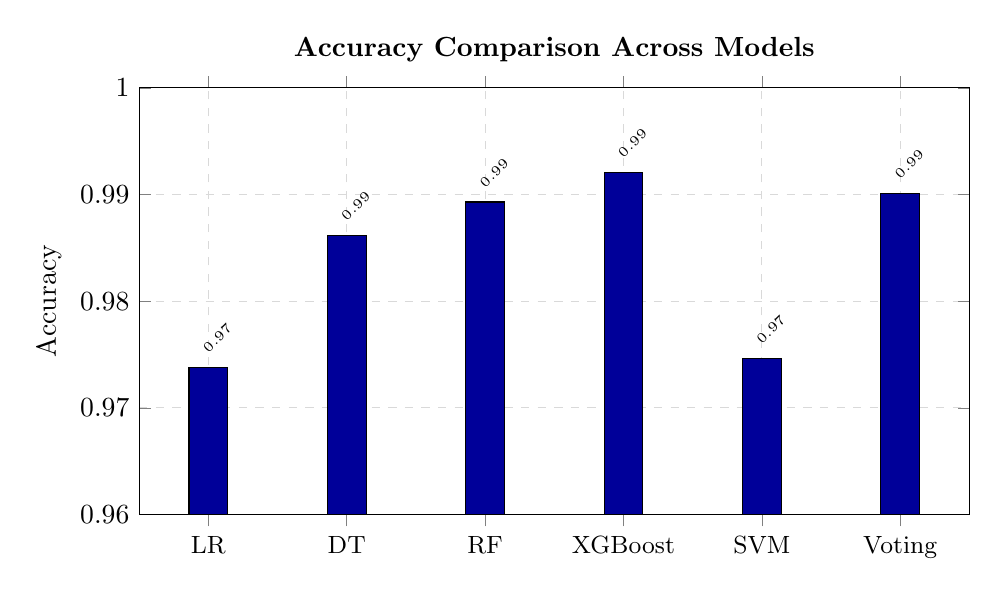
\begin{tikzpicture}
\begin{axis}[
  ybar,
  bar width=14pt,
  width=\textwidth,
  height=7cm,
  ylabel={Accuracy},
  ymin=0.96, ymax=1.0,
  symbolic x coords={LR, DT, RF, XGBoost, SVM, Voting},
  xtick=data,
  x tick label style={font=\small},
  nodes near coords,
  nodes near coords style={font=\tiny, above},
  every node near coord/.append style={rotate=45, anchor=south west},
  grid=major,
  grid style={dashed, gray!30},
  title={\textbf{Accuracy Comparison Across Models}},
  title style={font=\normalsize},
]
\addplot[fill=blue!60!black] coordinates {
  (LR, 0.9738)
  (DT, 0.9862)
  (RF, 0.9893)
  (XGBoost, 0.9921)
  (SVM, 0.9746)
  (Voting, 0.9901)
};
\end{axis}
\end{tikzpicture}
\caption{Accuracy comparison of all six candidates. XGBoost achieves the highest
accuracy (99.21\%), followed closely by the Voting Ensemble (99.01\%) and Random
Forest (98.93\%). Logistic Regression and SVM trail due to lower recall on minority
classes.}
\label{fig:acc-bar}
\end{figure}

% --- Figure: Macro-F1 Comparison ---
\begin{figure}[H]
\centering
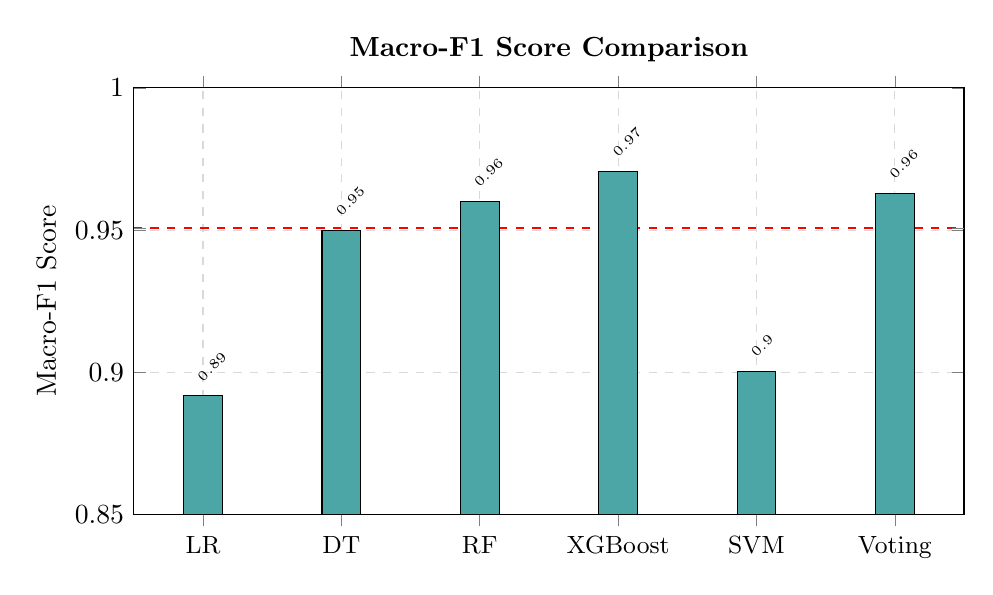
\begin{tikzpicture}
\begin{axis}[
  ybar,
  bar width=14pt,
  width=\textwidth,
  height=7cm,
  ylabel={Macro-F1 Score},
  ymin=0.85, ymax=1.0,
  symbolic x coords={LR, DT, RF, XGBoost, SVM, Voting},
  xtick=data,
  x tick label style={font=\small},
  nodes near coords,
  nodes near coords style={font=\tiny, above},
  every node near coord/.append style={rotate=45, anchor=south west},
  grid=major,
  grid style={dashed, gray!30},
  title={\textbf{Macro-F1 Score Comparison}},
  title style={font=\normalsize},
  % draw tolerance band
  extra y ticks={0.9506},
  extra y tick labels={},
  extra y tick style={grid=major, grid style={red, thick, dashed}},
]
\addplot[fill=teal!70] coordinates {
  (LR, 0.8917)
  (DT, 0.9500)
  (RF, 0.9600)
  (XGBoost, 0.9706)
  (SVM, 0.9002)
  (Voting, 0.9629)
};
\end{axis}
\end{tikzpicture}
\caption{Macro-F1 scores with the 2\,pp tolerance-band threshold at 0.9506 (dashed
red line). Three candidates --- RF, XGBoost, Voting --- clear the band; the Decision
Tree falls just 0.0006 short. Among the qualified trio, XGBoost leads.}
\label{fig:f1-bar}
\end{figure}

% --- Figure: Precision vs Recall (Grouped Bar) ---
\begin{figure}[H]
\centering
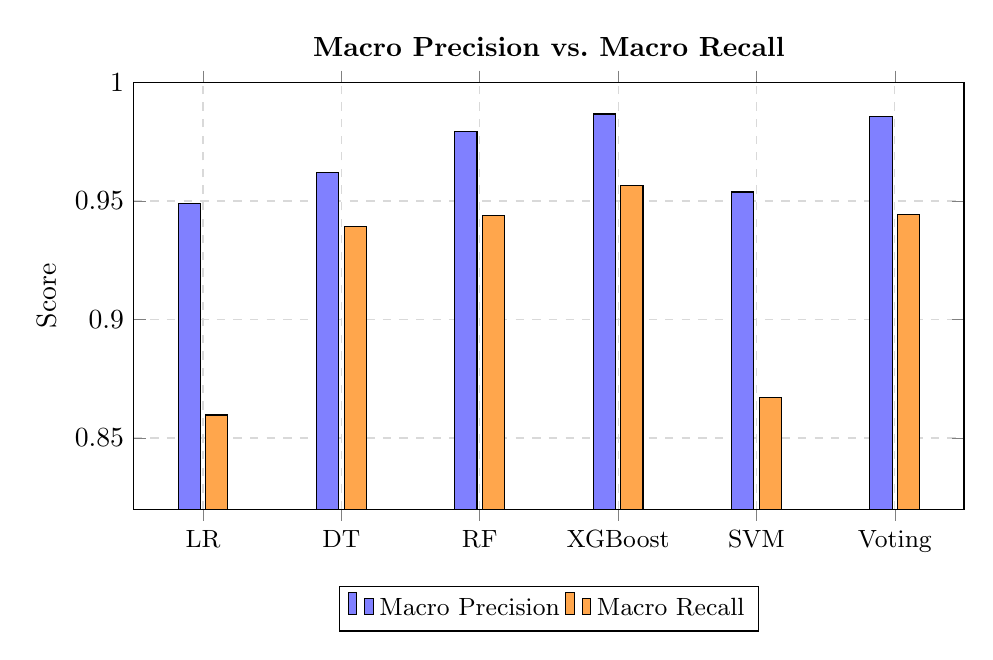
\begin{tikzpicture}
\begin{axis}[
  ybar,
  bar width=8pt,
  width=\textwidth,
  height=7cm,
  ylabel={Score},
  ymin=0.82, ymax=1.0,
  symbolic x coords={LR, DT, RF, XGBoost, SVM, Voting},
  xtick=data,
  x tick label style={font=\small},
  legend style={at={(0.5,-0.18)}, anchor=north, legend columns=2, font=\small},
  grid=major,
  grid style={dashed, gray!30},
  title={\textbf{Macro Precision vs.\ Macro Recall}},
  title style={font=\normalsize},
]
\addplot[fill=blue!50] coordinates {
  (LR, 0.9488)
  (DT, 0.9621)
  (RF, 0.9795)
  (XGBoost, 0.9867)
  (SVM, 0.9538)
  (Voting, 0.9856)
};
\addplot[fill=orange!70] coordinates {
  (LR, 0.8597)
  (DT, 0.9393)
  (RF, 0.9438)
  (XGBoost, 0.9566)
  (SVM, 0.8671)
  (Voting, 0.9443)
};
\legend{Macro Precision, Macro Recall}
\end{axis}
\end{tikzpicture}
\caption{Precision--recall trade-off by candidate. Models with high precision but
noticeably lower recall (LR, SVM) miss more attacks in the rare Authentication
class. XGBoost and the Voting Ensemble maintain the tightest gap, indicating
balanced performance across all four classes.}
\label{fig:prec-recall}
\end{figure}

% --- Figure: ROC-AUC Comparison ---
\begin{figure}[H]
\centering
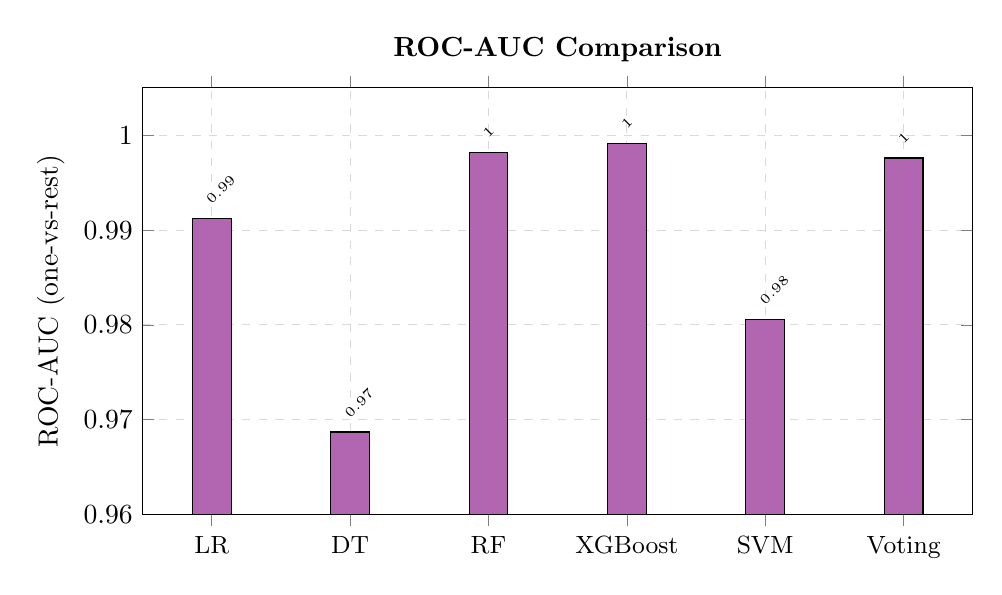
\begin{tikzpicture}
\begin{axis}[
  ybar,
  bar width=14pt,
  width=\textwidth,
  height=7cm,
  ylabel={ROC-AUC (one-vs-rest)},
  ymin=0.96, ymax=1.005,
  symbolic x coords={LR, DT, RF, XGBoost, SVM, Voting},
  xtick=data,
  x tick label style={font=\small},
  nodes near coords,
  nodes near coords style={font=\tiny, above},
  every node near coord/.append style={rotate=45, anchor=south west},
  grid=major,
  grid style={dashed, gray!30},
  title={\textbf{ROC-AUC Comparison}},
  title style={font=\normalsize},
]
\addplot[fill=violet!60] coordinates {
  (LR, 0.9912)
  (DT, 0.9687)
  (RF, 0.9982)
  (XGBoost, 0.9991)
  (SVM, 0.9806)
  (Voting, 0.9976)
};
\end{axis}
\end{tikzpicture}
\caption{ROC-AUC (one-vs-rest). XGBoost (0.9991) and Random Forest (0.9982) are
near-perfect rankers. The Decision Tree's lower AUC (0.9687) reflects its lack of
probability calibration --- hard splits produce step-function ROC curves.}
\label{fig:roc-bar}
\end{figure}

% --- Figure: Inference Latency Comparison (log scale) ---
\begin{figure}[H]
\centering
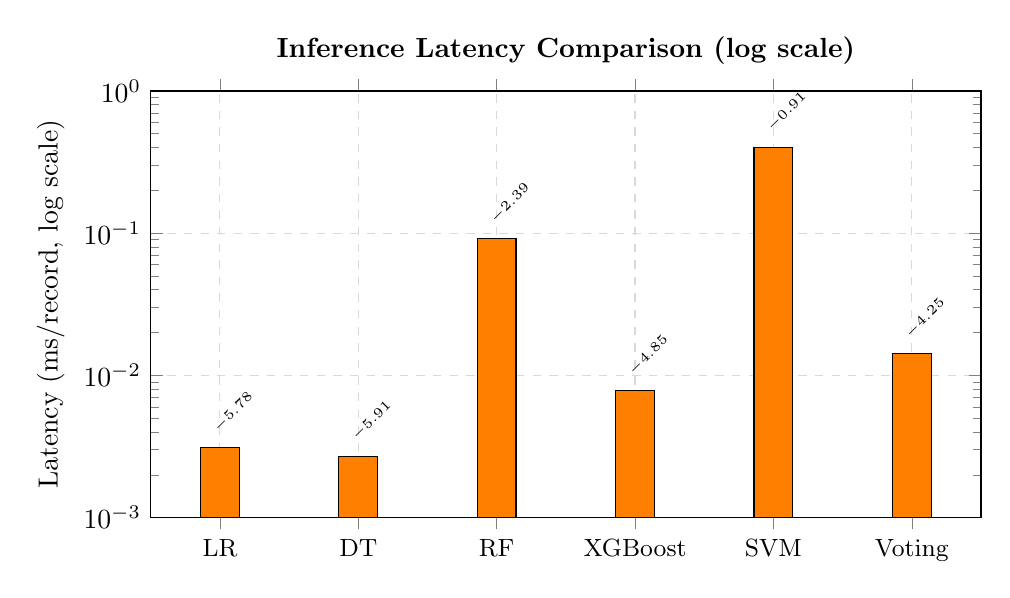
\begin{tikzpicture}
\begin{axis}[
  ybar,
  bar width=14pt,
  width=\textwidth,
  height=7cm,
  ylabel={Latency (ms/record, log scale)},
  ymode=log,
  log origin=infty,
  ymin=0.001, ymax=1,
  symbolic x coords={LR, DT, RF, XGBoost, SVM, Voting},
  xtick=data,
  x tick label style={font=\small},
  nodes near coords,
  nodes near coords style={font=\tiny, above},
  every node near coord/.append style={rotate=45, anchor=south west},
  grid=major,
  grid style={dashed, gray!30},
  title={\textbf{Inference Latency Comparison (log scale)}},
  title style={font=\normalsize},
]
\addplot[fill=red!50!yellow] coordinates {
  (LR, 0.0031)
  (DT, 0.0027)
  (RF, 0.0913)
  (XGBoost, 0.0078)
  (SVM, 0.4018)
  (Voting, 0.0142)
};
\end{axis}
\end{tikzpicture}
\caption{Per-record inference latency on a logarithmic scale. SVM is two orders of
magnitude slower than the tree-based models because each prediction requires a
kernel evaluation against all support vectors. Among the tolerance-band qualifiers,
XGBoost (0.0078\,ms) is roughly 2$\times$ faster than the Voting Ensemble
(0.0142\,ms) and 12$\times$ faster than Random Forest (0.0913\,ms).}
\label{fig:latency-bar}
\end{figure}

% --- Figure: Model Size Comparison (log scale) ---
\begin{figure}[H]
\centering
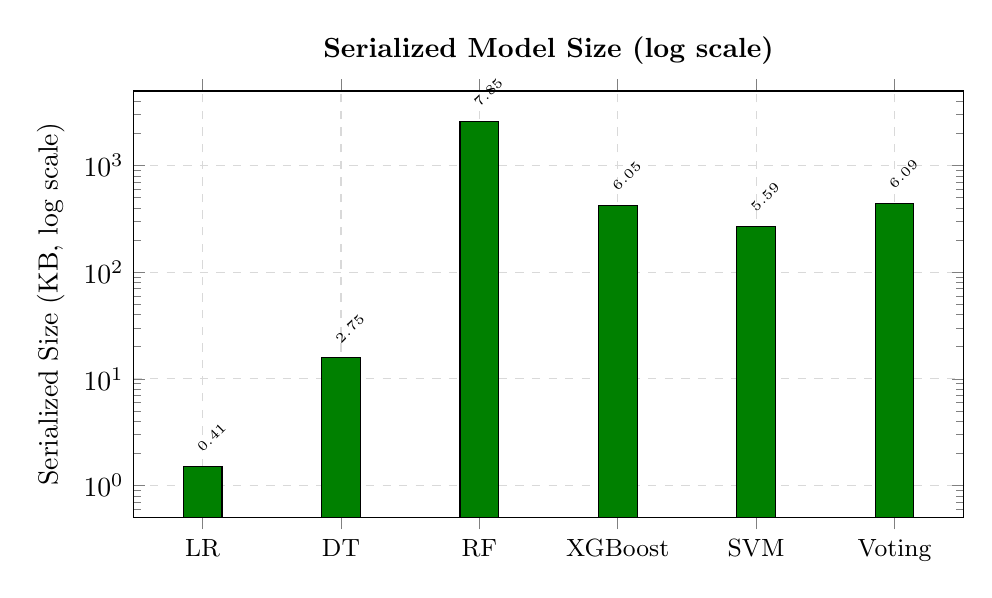
\begin{tikzpicture}
\begin{axis}[
  ybar,
  bar width=14pt,
  width=\textwidth,
  height=7cm,
  ylabel={Serialized Size (KB, log scale)},
  ymode=log,
  log origin=infty,
  ymin=0.5, ymax=5000,
  symbolic x coords={LR, DT, RF, XGBoost, SVM, Voting},
  xtick=data,
  x tick label style={font=\small},
  nodes near coords,
  nodes near coords style={font=\tiny, above},
  every node near coord/.append style={rotate=45, anchor=south west},
  grid=major,
  grid style={dashed, gray!30},
  title={\textbf{Serialized Model Size (log scale)}},
  title style={font=\normalsize},
]
\addplot[fill=green!50!black] coordinates {
  (LR, 1.5)
  (DT, 15.7)
  (RF, 2571)
  (XGBoost, 424)
  (SVM, 269)
  (Voting, 441)
};
\end{axis}
\end{tikzpicture}
\caption{Serialized model size. Linear models (LR: 1.5\,KB) and single trees (DT:
15.7\,KB) are tiny but less accurate. Random Forest is the largest at 2,571\,KB
(200 trees stored in full). XGBoost (424\,KB) offers the best accuracy-to-size
ratio among the qualified candidates.}
\label{fig:size-bar}
\end{figure}

Figures~\ref{fig:acc-bar}--\ref{fig:size-bar} visualize the key trade-offs that the
selection rule navigates. The accuracy and macro-F1 charts
(Figures~\ref{fig:acc-bar}--\ref{fig:f1-bar}) show that all six candidates exceed
97\% accuracy, but the spread in macro-F1 is much wider because macro-averaging
exposing weakness on minority classes. The precision--recall chart
(Figure~\ref{fig:prec-recall}) reveals the ``where'' of these weaknesses: LR and SVM
have acceptable precision but noticeably lower recall, meaning they miss attacks in
the small Authentication class. The ROC-AUC chart (Figure~\ref{fig:roc-bar}) confirms
that probability-based ranking quality is near-perfect for the ensemble and boosted
models. On the deployment-cost side, the latency chart (Figure~\ref{fig:latency-bar})
shows a two-order-of-magnitude spread and the size chart (Figure~\ref{fig:size-bar})
a three-order spread, underscoring why the selection rule must jointly weigh accuracy
and cost rather than optimizing either in isolation.

\subsection{Discussion and Limitations}
\begin{itemize}
  \item The primary deployment study runs on the \textbf{synthetic} generator; the
        real-data validation of Section~7.4 uses CIC-IDS-2017 (a PC-era IDS
        benchmark), so absolute numbers may still not transfer to constrained IoT
        gateways or to TON\_IoT-style telemetry.
  \item The live-accuracy figure is based on a small first sample (141 records) and
        should be re-measured over longer runs.
  \item Drift signalling (e.g., population-stability index) and retraining triggers
        are not yet implemented.
  \item The CPU figure includes the whole Flask process and is not equivalent to the
        paper's dedicated-node measurement.
\end{itemize}

%====================================================================
% 8. GRAPHICAL USER INTERFACE
%====================================================================
\clearpage
\section{Graphical User Interface}

The dashboard is a monochrome single-page app (dark by default, an equivalent light
theme, and a single red accent for attacks); the theme choice persists and charts
re-render in place. It has five pages: Overview, Model Lab, Live Detection,
Investigate Device and How It Works --- summarized in Table~\ref{tab:gui}, followed by
annotated screenshots.

\begingroup
\small
\renewcommand{\arraystretch}{1.2}
\begin{longtable}{@{}>{\raggedright\arraybackslash}p{2.6cm}
                   >{\raggedright\arraybackslash}p{7.2cm}
                   >{\raggedright\arraybackslash}p{5.2cm}@{}}
\caption{GUI pages and their purpose}\label{tab:gui}\\
\toprule
\textbf{Page} & \textbf{Key elements} & \textbf{Purpose}\\
\midrule
\endfirsthead
\toprule
\textbf{Page} & \textbf{Key elements} & \textbf{Purpose}\\
\midrule
\endhead
\bottomrule
\endfoot
\bottomrule
\endlastfoot
\textbf{Overview} & Records processed, attacks detected, average edge latency; deployed model card; live accuracy; fog-node CPU/RSS/threads; Start/Pause/Reset; speed 1x/5x/20x; attack-type distribution; traffic over time & Mission control: what is deployed and what it is catching now\\
\textbf{Model Lab} & Train Models; deployment banner (RULE AUTOMATIC / MANUAL OVERRIDE); tolerance slider 0--10 pp; tiebreaker selector; variant toggle full vs PCA; comparison table with per-row Deploy; latency-vs-F1 scatter; PCA charts; selection reasoning panel; confusion-matrix heatmap & The cloud role: train, compare, explore the rule\\
\textbf{Live Detection} & Start/Stop simulator and RUNNING badge; class tally; DBSCAN window scatter; filter bar (class checkboxes and IP search); live feed with class, confidence and latency & The fog role: watch classification and the anomaly backstop\\
\textbf{Investigate Device} & IP search; top-40 devices by volume; classification timeline (one dot per event); class breakdown; last 30 events & Per-device behaviour story\\
\textbf{How It Works} & Six cards mapping each CSC701 module to the implementing component & Static reference\\
\end{longtable}
\endgroup

\begin{figure}[H]
  \centering
  \figplaceholder{images/fig3_overview.png}{0.8\textwidth}{Overview page: counters, deployed model card, live accuracy, fog resources}
  \caption{Overview page}
  \label{fig:overview}
\end{figure}

\begin{figure}[H]
  \centering
  \figplaceholder{images/fig4_attack_dist.png}{0.8\textwidth}{Attack-type distribution and traffic-over-time charts}
  \caption{Attack-type distribution and traffic over time}
  \label{fig:attackdist}
\end{figure}

\begin{figure}[H]
  \centering
  \figplaceholder{images/fig5_traffic_class.png}{0.8\textwidth}{Traffic over time by class (line styles per class)}
  \caption{Traffic over time by class}
  \label{fig:trafficclass}
\end{figure}

\begin{figure}[H]
  \centering
  \figplaceholder{images/fig6_comparison.png}{0.8\textwidth}{Candidate comparison table with IN BAND outlines and RULE PICK}
  \caption{Model Lab: candidate comparison table}
  \label{fig:comparison}
\end{figure}

\begin{figure}[H]
  \centering
  \figplaceholder{images/fig7_latency_f1.png}{0.75\textwidth}{Latency vs macro-F1 scatter with shaded tolerance band}
  \caption{Latency versus macro-F1 with tolerance band}
  \label{fig:latf1}
\end{figure}

\begin{figure}[H]
  \centering
  \figplaceholder{images/fig8_pca_variance.png}{0.75\textwidth}{PCA cumulative-variance chart with 95\% target line}
  \caption{PCA cumulative variance}
  \label{fig:pcavar}
\end{figure}

\begin{figure}[H]
  \centering
  \figplaceholder{images/fig9_confusion.png}{0.62\textwidth}{Confusion-matrix heatmap of the deployed model}
  \caption{Confusion matrix of the deployed XGBoost model}
  \label{fig:cm}
\end{figure}

\begin{figure}[H]
  \centering
  \figplaceholder{images/fig10_dbscan.png}{0.75\textwidth}{DBSCAN window scatter (2D projection, anomalies in red)}
  \caption{DBSCAN window scatter}
  \label{fig:dbscan}
\end{figure}

\begin{figure}[H]
  \centering
  \figplaceholder{images/fig11_live_feed.png}{0.75\textwidth}{Live feed with predicted class, confidence and latency}
  \caption{Live Detection feed}
  \label{fig:livefeed}
\end{figure}

\begin{figure}[H]
  \centering
  \figplaceholder{images/fig12_device.png}{0.8\textwidth}{Device classification timeline}
  \caption{Investigate Device timeline}
  \label{fig:device}
\end{figure}

\begin{figure}[H]
  \centering
  \figplaceholder{images/fig13_themes.png}{0.8\textwidth}{Light and dark theme comparison}
  \caption{Light and dark themes}
  \label{fig:themes}
\end{figure}

%====================================================================
% 9. CODE
%====================================================================
\clearpage
\section{Code (Libraries and Functions Used)}

The full source is in the project repository; the listings below show the key parts
of each mechanism.

\subsection{Model Training and Uniform Evaluation}
\begin{lstlisting}
from sklearn.linear_model import LogisticRegression
from sklearn.tree import DecisionTreeClassifier
from sklearn.ensemble import RandomForestClassifier, VotingClassifier
from sklearn.svm import SVC
from xgboost import XGBClassifier

CANDIDATES = {
    "Logistic Regression": lambda: LogisticRegression(max_iter=2000),
    "Decision Tree":       lambda: DecisionTreeClassifier(random_state=42),
    "Random Forest":       lambda: RandomForestClassifier(n_estimators=200, random_state=42),
    "XGBoost":             lambda: XGBClassifier(random_state=42, eval_metric="mlogloss"),
    "SVM (RBF)":           lambda: SVC(kernel="rbf", probability=True),
    "Voting (LR+DT+XGB)":  lambda: VotingClassifier(
        estimators=[("lr", LogisticRegression(max_iter=2000)),
                    ("dt", DecisionTreeClassifier(random_state=42)),
                    ("xgb", XGBClassifier(random_state=42, eval_metric="mlogloss"))],
        voting="soft"),
}

def train_and_evaluate(X_train, X_test, y_train, y_test, tolerance=0.02):
    results = []
    for name, factory in CANDIDATES.items():
        model = factory().fit(X_train, y_train)
        y_pred = model.predict(X_test)
        results.append(measure(name, model, y_test, y_pred))
    return select_deployment(results, tolerance)
\end{lstlisting}

\subsection{The Selection Rule}
\begin{lstlisting}
best_f1   = max(c.macro_f1 for c in candidates)
qualified = [c for c in candidates
             if c.macro_f1 >= best_f1 - tolerance]   # default tolerance = 0.02
winner    = min(qualified, key=tiebreaker)           # default: latency (ms/record)
\end{lstlisting}

\subsection{PCA Evaluation and Adoption Rule}
\begin{lstlisting}
pca = PCA(n_components=0.95, random_state=42)   # keep >=95% variance
X_train_r = pca.fit_transform(X_train)
X_test_r  = pca.transform(X_test)

f1_cost = full.macro_f1 - reduced.macro_f1
adopt_pca = (f1_cost <= 0.01) and (reduced.latency <= full.latency)
variant = "pca_reduced" if adopt_pca else "full_features"
\end{lstlisting}

\subsection{Export and Edge Loading}
\begin{lstlisting}
import joblib

# Cloud: export the winning pipeline plus metadata
joblib.dump({"pipeline": winner_pipeline,
             "classes": class_map,
             "reasoning": reasoning},
            "artifacts/deployed_model.joblib", compress=3)

# Fog: load only the artifact (no training stack needed)
artifact = joblib.load("artifacts/deployed_model.joblib")
pred = artifact["pipeline"].predict(record)
\end{lstlisting}

\subsection{DBSCAN Anomaly Backstop}
\begin{lstlisting}
from sklearn.cluster import DBSCAN

def backstop(window):                    # rolling 1,500 standardized records
    labels = DBSCAN(eps=1.8, min_samples=8).fit_predict(window)
    anomalies = window[labels == -1]    # noise = unknown traffic
    return anomalies
\end{lstlisting}

%====================================================================
% 10. CONCLUSION
%====================================================================
\clearpage
\section{Conclusion}
SentryMesh operationalizes the paper's ``search in the cloud, serve at the fog'' idea
as a working, explainable system. Six architecturally different candidates were
compared under one harness, and an explicit tolerance-band rule chose \textbf{XGBoost}
(macro-F1 0.9706, kappa 0.9821, ROC-AUC 0.9991, 424\,KB, about 0.01\,ms per record),
rejecting the cheapest model for missing the accuracy band and the ensembles for
higher latency. A data-driven PCA test showed dimensionality reduction was not worth
a 0.24 macro-F1 loss. The fog tier generalized to a separate drifted distribution
(99.3\% live versus 99.21\% test accuracy), added a DBSCAN backstop for zero-day
traffic, and reported its own latency and CPU/memory use.

\textbf{Limitations:} synthetic data for the deployment study, a small live-accuracy
sample, CPU measured on the whole development process rather than a constrained
node, and a real-data validation limited to three classes (CIC-IDS-2017's local
copy covers no credential-attack days, so the Authentication class is exercised
only in the synthetic study).

\textbf{Future work:} a drift indicator (PSI) with a retraining trigger;
CPU-constrained or Raspberry Pi fog deployment; real testbed capture (Fed4Fire,
COSMOS, POWDER); TON\_IoT/CICIoT2023 runs to restore the four-class taxonomy on real
traffic; cross-dataset drift tests (train CIC-IDS-2017, test CICIDS2018); and an
XGBoost hyperparameter grid in the cloud tier.

%====================================================================
% 11. REFERENCES
%====================================================================
\clearpage
\begin{thebibliography}{99}
\addcontentsline{toc}{section}{References}
\renewcommand{\refname}{References}

\bibitem{ref1} V.~Tomer and S.~Sharma (2022). Detecting IoT Attacks Using an Ensemble Machine Learning Model. \textit{Future Internet}, 14(4), 102. doi:10.3390/fi14040102.

\bibitem{ref2} T.~Chen and C.~Guestrin (2016). XGBoost: A scalable tree boosting system. In \textit{Proceedings of the 22nd ACM SIGKDD International Conference on Knowledge Discovery and Data Mining} (pp. 785--794).

\bibitem{ref3} F.~Pedregosa \textit{et al.} (2011). Scikit-learn: Machine learning in Python. \textit{Journal of Machine Learning Research}, 12, 2825--2830.

\bibitem{ref4} M.~Ester, H.-P. Kriegel, J.~Sander, and X.~Xu (1996). A density-based algorithm for discovering clusters in large spatial databases with noise. In \textit{Proceedings of KDD-96} (pp. 226--231).

\bibitem{ref5} A.~Alsaedi, N.~Moustafa, Z.~Tari, A.~Mahmood, and A.~Anwar (2020). TON\_IoT telemetry dataset: A new generation dataset of IoT and IIoT for data-driven intrusion detection systems. \textit{IEEE Access}, 8, 165130--165150. doi:10.1109/ACCESS.2020.3022862.

\bibitem{ref6} E.~C.~P. Neto, S.~Dadkhah, R.~Ferreira, A.~Zohourian, R.~Lu, and A.~A. Ghorbani (2023). CICIoT2023: A real-time dataset and benchmark for large-scale attacks in IoT environment. \textit{Sensors}, 23(13), 5941. doi:10.3390/s23135941.

\bibitem{ref7} University of Mumbai, CSC701 Machine Learning syllabus (Rev-2019 `C' Scheme), Modules 2--4 and 6.

\bibitem{ref8} Project documents: \texttt{SentryMesh-ML-PRD.md}, \texttt{PAPER\_REVIEW.md}, \texttt{README.md}, \texttt{REPORT.md}.

\bibitem{ref9} I.~Sharafaldin, A.~H.~Lashkari, and A.~A.~Ghorbani (2018). Toward generating a new intrusion detection dataset and intrusion traffic characterization. In \textit{Proceedings of the 4th International Conference on Information Systems Security and Privacy (ICISSP)} (pp. 108--116). doi:10.5220/0006639801080116.

\end{thebibliography}

\end{document}
